\subsection{Model}
  \label{subsection:model}

As mentioned by Krasner and Pope \autocite{krasner-pope-88}, an application's model is a domain specific simulation or implementation of a structure. The model component of an MVC application contains business logic and manages the state of an application as well as its storage. 
The essential models of the system can be defined by revisiting the sequences listed on \autoref{section:sequence} and identifying the important structures needed to fulfill the requirements needed.
  
\subsubsection{Validation Rule}
Through a detailed analysis of the sequence listed on \autoref{subsection:seq-notification}, it is essential that the \emph{validation rule} model contains the following attributes:

\begin{itemize}
  \item A URL pointing to an external endpoint
  \item A list of conditions to evaluate the response returned by the external endpoint
  \item A unique identifier
  \item A fail score, which determine the severity of the rule if the evaluation failed
\end{itemize}

It might also be necessary to have an identifier in the validation rule to skip its evaluation in certain cases. Other than that, as the FDS would make an HTTP request to an external endpoint based on the information listed on a validation rule, the following attributes are needed to provide a more robust configuration:

\begin{itemize}
  \item HTTP method to be used to make the request
  \item Request header\footnote{In \autocite[\enquote{5.3 Request Header Fields}]{http-rfc}: request header is defined as additional information passed by the client to the host server about the particular request or about the client.}
  \item Request body
\end{itemize}

As the FDS interacts with external endpoints, there is no guarantee that the external endpoint will always be accessible. An additional attribute to specify and configure a retry strategy in such cases can be useful. However, a retry strategy can be really specific to its implementation and therefore will be discussed in \textbf{TODO: Add retry strategy implementation}.

An additional \emph{priority} attribute is also provided to enable the possibility to run rule validations according to its priority order.

\begin{figure}[!h]
  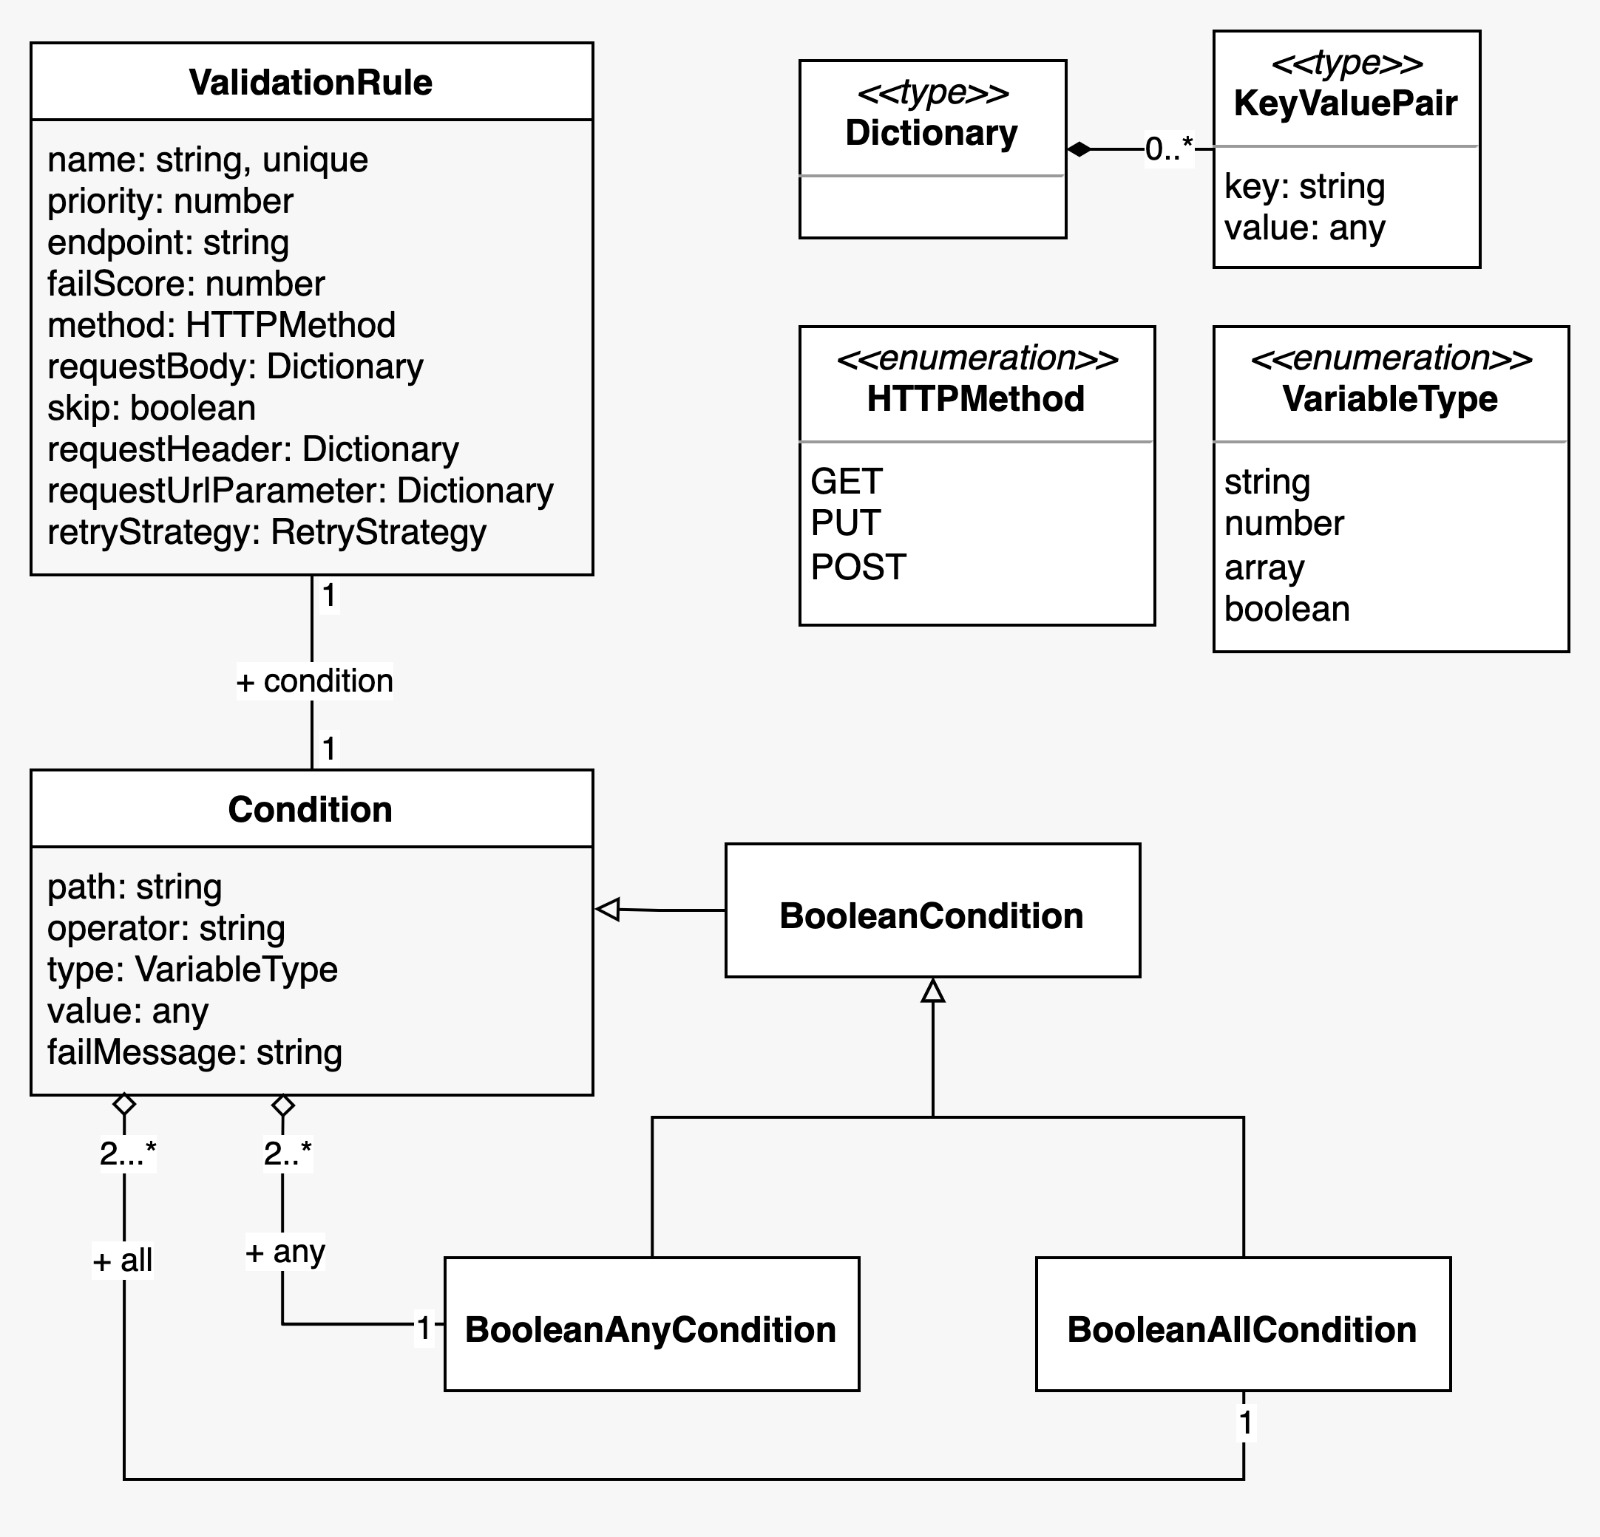
\includegraphics[width=\textwidth]{diagrams/entity_validation_rule.jpeg}
  \caption{UML diagram of the validation rule model}
 \end{figure}
 
The \emph{condition} attribute plays an important role for a validation rule, as it defines how the response returned by the external endpoint should be to pass a rule evaluation. It is intended to design the condition attribute to be robust and configurable. The \emph{path} of a condition defines a JSONPath\autocite{Friesen2019} expression to access information available of the current validation scope, such as customer information or response returned by the external endpoint. The \emph{type} attribute of a condition determines the type of the attribute accessed by the \emph{path} attribute. The \emph{type} attribute determines which type of operators are available to use\footnote{For example: a condition with \emph{type} "string" cannot use the "incl" \emph{operator}, because the "incl" \emph{operator} is only available for "array" \emph{type}}. The \emph{operator} attribute refers to a name of operator to be used to evaluate the condition (for example: "eq", "incl"). The available operator names are predefined and restricted to the condition's type attribute. More information regarding operators will be discussed in \textbf{TODO: Add retry strategy implementation} % ANCHOR: CHECKPOINT

\subsubsection{Validation Result}